\part{JavaScript}

\newpage

\chapter{JavaScript简介}

\section{编程简介}

\subsection{编程简介}

程序(program)是为了让计算机执行某些操作或者解决问题而编写的一系列有序指令的集合。由于计算机只能够识别二进制数字0和1,因此需要使用特殊的编程语言来描述如何解决问题过程和方法。 \\

算法(algorithm)是可完成特定任务的一系列步骤,算法的计算过程定义明确,通过一些值作为输入并产生一些值作为输出。 \\

流程图(flow chart)是算法的一种图形化表示方式,使用一组预定义的符号来说明如何执行特定任务。 \\

\begin{itemize}
	\item 圆角矩形:开始和结束
	\item 矩形:数据处理
	\item 平行四边形:输入/输出
	\item 菱形:分支判断条件
	\item 流程线:步骤
\end{itemize}

\begin{figure}
	\centering
	\begin{tikzpicture}[node distance=2cm]
		\node (start) [startend] {Start};
		\node (init)   [io, below of=start] {$ i = 0 $, $ sum = 0 $};
		\node (decision)  [decision, below of=init] {$ i \le 100 $?};
		\node (accumulation) [process, below of=decision] {$ sum = sum + i $};
		\node (update) [process, below of=accumulation] {$ i = i + 1 $};
		\node (output) [io, right of=decision, xshift=2.5cm] {print $ sum $};
		\node (end) [startend, below of=update] {End};

		\draw [arrow] (start) -- (init);
		\draw [arrow] (init) -- (decision);
		\draw [arrow] (decision) -- node[anchor=east] {yes } (accumulation);
		\draw [arrow] (accumulation) -- (update);
		\draw [arrow] (update) -- (-3,-8) -- (-3,-4) -- (decision);
		\draw [arrow] (decision) -- node[anchor=south] {no} (output);
		\draw [arrow] (output) |- (end);
	\end{tikzpicture}
	\caption{计算$ \sum_{i=1}^{100} i $的流程图}
\end{figure}

\subsection{编程语言(Programming Language)}

编程语言主要分为面向机器、面向过程和面向对象三类。JavaScript是一种具有函数优先的轻量级,解释型或即时编译型的编程语言。虽然它是作为开发Web页面的脚本语言而出名,但是它也被用到了很多非浏览器环境中。JavaScript基于原型编程、多范式的动态脚本语言,并且支持面向对象、命令式、声明式、函数式编程范式。

\begin{figure}[H]
	\centering
	
\includegraphics[scale=0.9]{img/C9/9-1/1.png}
\end{figure}

\section{Hello World!}

\subsection{Hello World!}

使用\lstinline|<script>|在HTML网页中插入JavaScript代码。 \\

\begin{lstlisting}[style=htmlcssjs]
<script type="text/JavaScript">
    // JavaScript代码
</script>
\end{lstlisting}

type属性表示在\lstinline|<script>|之间的是文本类型,告诉了浏览器里面的文本属于JavaScript语言。 \\

JS作为一种脚本语言可以放在HTML页面中任何位置,但是一般放在网页的\lstinline|<head>|或\lstinline|<body>|部分。最常用的方式是在页面\lstinline|<head>|部分放置\lstinline|<script>|元素,浏览器解析HTML时是按先后顺序的,所以前面的\lstinline|<script>|就先被执行。 \\

\subsection{引入外部JS文件}

除了在HTML文件中使用\lstinline|<script>|添加JS代码,还能把HTML和JS分开,单独创建一个JS文件,其文件后缀为“.js”,然后直接将JS代码写在JS文件中。注意在JS文件中,不需要\lstinline|<script>|,直接编写JS代码即可。 \\

JS文件不能直接运行,需要嵌入到HTML文件中执行,因此需要在HTML中引入外部JS文件。 \\

\begin{lstlisting}[style=htmlcssjs]
<script src="JS文件.js"></script>
\end{lstlisting}

\mybox{Hello World!}

\begin{lstlisting}[style=htmlcssjs, title=hello\_world.html]
<!DOCTYPE html>
<html lang="en">
<head>
    <meta charset="UTF-8">
    <title>Hello World!</title>
    <script src="hello_world.js"></script>
</head>
<body>

</body>
</html>
\end{lstlisting}

\begin{lstlisting}[style=htmlcssjs, title=hello\_world.js]
document.write("Hello World!");
\end{lstlisting}

\newpage

\section{语句与注释}

\subsection{语句(Statement)}

JS语句是发给浏览器的命令,这些命令的作用是告诉浏览器要做的事情。一行语句通常在结尾加上一个【;】表示语句的结束,虽然分号也可以不写,但是要养成编程的好习惯,记得在语句末尾加上分号。

\subsection{注释(Comment)}

在编程中加入注释可以增加程序的可读性和可维护性,编译器不会对注释的部分进行编译。 \\

JS中注释分为两类:

\begin{enumerate}
	\item 单行注释:将一行内【//】之后的内容视为注释。
	\item 多行注释:以【/*】开始,【*/】结束,中间的内容视为注释。
\end{enumerate}

\mybox{注释} \\

\begin{lstlisting}[style=htmlcssjs]
document.write("单行注释");     // 我是单行注释
/*
    我是
    多行
    注释
*/
document.write("多行注释");
\end{lstlisting}

\newpage

\section{互动方法}

\subsection{document.write()}

\lstinline|document.write()|可用于直接向HTML输出流写内容,简单地说就是直接在网页中输出内容。 \\

\begin{lstlisting}[style=htmlcssjs]
document.write("互动方法:document.write()");
\end{lstlisting}

\subsection{console.log()}

\lstinline|console.log()|用于在控制台输出信息,该方法对于开发过程进行测试很有帮助。 \\

\begin{lstlisting}[style=htmlcssjs]
console.log("互动方法:console.log()");
\end{lstlisting}

\subsection{alert()}

在访问网站的时候,有时会突然弹出一个小窗口,上面写着一段提示信息文字,如果不点击“确定”,就不能对网页做任何操作,这个小窗口就是使用\lstinline|alert()|实现的。 \\

\begin{lstlisting}[style=htmlcssjs]
alert("互动方法:alert()");
\end{lstlisting}

\subsection{confirm()}

\lstinline|confirm()|消息对话框通常用于允许用户做选择的动作,弹出对话框包含一个确定按钮和一个取消按钮。 \\

\lstinline|confirm()|的返回值为boolean值,当用户点击“确定”按钮时返回true,当用户点击“取消”按钮时返回false。 \\

\begin{lstlisting}[style=htmlcssjs]
confirm("互动方法:confirm()");
\end{lstlisting}

\subsection{prompt()}

\lstinline|prompt()|弹出消息对话框,通常用于询问一些需要与用户交互的信息,弹出的消息对话框包含一个确定按钮、取消按钮和一个文本输入框。 \\

\lstinline|prompt()|接受两个参数,第一个参数为要显示在消息对话框中的文本,不可修改;第二个参数为文本框中的内容,可以修改。点击“确定”按钮,文本框中的内容将作为函数的返回值;点击“取消”按钮,将返回null。 \\

\begin{lstlisting}[style=htmlcssjs]
prompt("互动方法:prompt()", "文本内容");
\end{lstlisting}

\newpage

\section{变量}

\subsection{变量(Variable)}

变量是计算机中一块特定的内存空间,由一个或多个连续的字节组成,不同数据存入具有不同内存地址的空间,相互独立,通过变量名可以简单快速地找到在内存中存储的数据。定义变量使用关键字var。 \\

\begin{lstlisting}[style=htmlcssjs]
var variable_name;
\end{lstlisting}

变量名需要符合以下的要求:

\begin{enumerate}
	\item 由字母、数字和下划线组成,第一个字符必须为字母或下划线。
	\item 不能包含除【\_】以外的任何特殊字符,如【\%】、【\#】等。
	\item 不可以使用保留字或关键字。
	\item 准确、顾名思义,不要使用汉语拼音。
\end{enumerate}

关键字是编程语言内置的一些名称,具有特殊的用处和意义。

\begin{table}[H]
	\centering
	\setlength{\tabcolsep}{5mm}{
		\begin{tabular}{|c|c|c|c|c|}
			\hline
			break        & else       & new       & var       & case       \\
			\hline
			finally      & return     & void      & catch     & for        \\
			\hline
			switch       & while      & default   & if        & throw      \\
			\hline
			do           & instanceof & typeof    & abstract  & enum       \\
			\hline
			short        & boolean    & export    & interface & static     \\
			\hline
			extends      & long       & super     & char      & final      \\
			\hline
			synchronized & class      & float     & package   & throws     \\
			\hline
			goto         & private    & transient & debugger  & implements \\
			\hline
			volatile     & double     & import    & public    & delete     \\
			\hline
			in           & try        & int       & byte      & native     \\
			\hline
			const        & protected  &           &           &            \\
			\hline
		\end{tabular}
	}
	\caption{关键字}
\end{table}

\subsection{初始化(Initialization)}

变量可以在定义时初始化,也可以在定义后初始化。 \\

在编程中,【=】不是数学中的“等于”符号,而是表示“赋值”,即将【=】右边的值赋给左边的变量。 \\

\begin{lstlisting}[style=htmlcssjs]
var n = 10;
var wage = 8232.56;
\end{lstlisting}

JS变量虽然也可以不声明直接使用,但是这样不规范。

\newpage

\section{数据类型}

\subsection{数据类型}

JS中变量主要有以下几种类型:

\begin{enumerate}
	\item 数字number:整型、浮点型
	\item 字符串string
	\item 布尔boolean
	\item 空对象null
	\item 未定义undefined
	\item 复杂数据类型:数组Array、对象Object
\end{enumerate}

使用\lstinline|typeof()|可以检测一个变量的数据类型。 \\

\mybox{数据类型} \\

\begin{lstlisting}[style=htmlcssjs]
var a = 12;
var b = 3.1415;
var c = "hello";
var d = false;

console.log(typeof(a))
console.log(typeof(b))
console.log(typeof(c))
console.log(typeof(d))
\end{lstlisting}

\begin{tcolorbox}
	\mybox{运行结果} \\
	number \\
	number \\
	string \\
	boolean
\end{tcolorbox}

\subsection{类型转换}

类型转换是把变量从一种类型转换为另一种数据类型。类型转换可以是隐式的,也可以是显式的,通过使用强制类型转换的方法来指定。 \\

\mybox{类型转换} \\

\begin{lstlisting}[style=htmlcssjs]
console.log(Number("123"));
console.log(parseInt("456"));
console.log(parseFloat("78.9"));
console.log(String(123456789));
console.log(Boolean(0));
console.log(Boolean(1));
\end{lstlisting}

\begin{tcolorbox}
	\mybox{运行结果} \\
	123 \\
	456 \\
	78.9 \\
	123456789 \\
	false \\
	true
\end{tcolorbox}

\newpage

\section{算术运算符}

\subsection{四则运算}

\begin{table}[H]
	\centering
	\setlength{\tabcolsep}{5mm}{
		\begin{tabular}{|c|c|c|}
			\hline
			\textbf{数学符号} & \textbf{JS符号} & \textbf{含义} \\
			\hline
			$ + $             & +               & 加法          \\
			\hline
			$ - $             & -               & 减法          \\
			\hline
			$ \times $        & *               & 乘法          \\
			\hline
			$ \div $          & /               & 除法          \\
			\hline
			$ \dots\dots $    & \%              & 取模          \\
			\hline
		\end{tabular}
	}
	\caption{四则运算}
\end{table}

JS中除法【/】的意义与数学中不同:

\begin{enumerate}
	\item 当相除的两个运算数都为整型,则运算结果为两个数进行除法运算后的整数部分,例如21 / 5的结果为4。

	\item 如果两个运算数其中至少一个为浮点型,则运算结果为浮点型,如21 / 5.0的结果为4.2。
\end{enumerate}

取模(modulo)【\%】表示求两个数相除之后的余数,如22 \% 3的结果为1;4 \% 7的结果为4。

\subsection{复合赋值运算符}

\begin{table}[H]
	\centering
	\setlength{\tabcolsep}{5mm}{
		\begin{tabular}{|c|c|}
			\hline
			\textbf{运算符} & \textbf{描述}                                        \\
			\hline
			+=              & \lstinline|a += b|等价于\lstinline|a = a + b| \\
			\hline
			-=              & \lstinline|a -= b|等价于\lstinline|a = a - b| \\
			\hline
			*=              & \lstinline|a *= b|等价于\lstinline|a = a * b| \\
			\hline
			/=              & \lstinline|a /= b|等价于\lstinline|a = a / b| \\
			\hline
			\%=             & \lstinline|a %= b|等价于\lstinline|a = a % b| \\
			\hline
		\end{tabular}
	}
	\caption{复合赋值运算符}
\end{table}

\newpage

\section{表达式}

\subsection{字符串连接}

【+】运算符不只代表加法,还可以用于连接两个字符串。 \\

\mybox{字符串连接} \\

\begin{lstlisting}[style=htmlcssjs]
console.log("Hello" + "World");
\end{lstlisting}

\begin{tcolorbox}
	\mybox{运行结果} \\
	HelloWorld
\end{tcolorbox}

\subsection{转义字符}

在一个字符串描述的过程中,有可能会有一些特殊字符的信息。

\begin{table}[H]
	\centering
	\setlength{\tabcolsep}{5mm}{
		\begin{tabular}{|c|c|}
			\hline
			\textbf{转义字符}       & \textbf{描述}                         \\
			\hline
			\lstinline|\\| & 表示一个反斜杠\lstinline|\| \\
			\hline
			\lstinline|\'| & 表示一个单引号\lstinline|'| \\
			\hline3
			\lstinline|\"| & 表示一个双引号\lstinline|"| \\
			\hline
			\lstinline|\n| & 换行                                  \\
			\hline
			\lstinline|\t| & 横向制表符                            \\
			\hline
		\end{tabular}
	}
	\caption{转义字符}
\end{table}

\mybox{转义字符} \\

\begin{lstlisting}[style=htmlcssjs]
console.log("全球最大同性交友网站\n\'https://github.com\'");
\end{lstlisting}

\begin{tcolorbox}
	\mybox{运行结果} \\
	全球最大同性交友网站 \\
	'https://github.com'
\end{tcolorbox}

\subsection{表达式(Expression)}

表达式与数学中的定义相似,表达式是值具有一定的值,用操作符把常数和变量连接起来的代数式。 \\

使用\lstinline|prompt()|可以获取用户输入的信息,返回值为字符串类型。 \\

\mybox{计算圆的面积} \\

\begin{lstlisting}[style=htmlcssjs]
var PI = 3.14159;
var r = parseFloat(prompt("输入半径"));
var area = PI * r ** 2;
console.log("面积 = " + area);
\end{lstlisting}

\begin{tcolorbox}
	\mybox{运行结果} \\
	输入半径:5 \\
	面积 = 78.53975
\end{tcolorbox}

\lstinline|Math.floor()|的作用是向下取整,\lstinline|Math.ceil()|的作用是向上取整。 \\

\mybox{逆序三位数} \\

\begin{lstlisting}[style=htmlcssjs]
var num = parseInt(prompt("输入一个正三位数"));
var a = Math.floor(num / 100);
var b = Math.floor(num / 10) % 10;
var c = num % 10;

num = c * 100 + b * 10 + a;
console.log("逆序:" + num);
\end{lstlisting}

\begin{tcolorbox}
	\mybox{运行结果} \\
	输入一个正三位数:520 \\
	逆序:25
\end{tcolorbox}

\newpage

\chapter{判断}

\section{逻辑运算符}

\subsection{关系运算符}

\begin{table}[H]
	\centering
	\setlength{\tabcolsep}{5mm}{
		\begin{tabular}{|c|c|}
			\hline
			\textbf{数学符号} & \textbf{关系运算符} \\
			\hline
			$ < $             & <                   \\
			\hline
			$ > $             & >                   \\
			\hline
			$ \le $           & <=                  \\
			\hline
			$ \ge $           & >=                  \\
			\hline
			$ \ne $           & !=                  \\
			\hline
			$ = $             & ==                  \\
			\hline
		\end{tabular}
	}
	\caption{关系运算符}
\end{table}

\subsection{逻辑运算符}

JS中逻辑运算符有三种:

\begin{enumerate}
	\item 逻辑与\&\&(logical AND):当多个条件同时为真,结果为真。
	      \begin{table}[H]
		      \centering
		      \setlength{\tabcolsep}{5mm}{
			      \begin{tabular}{|c|c|c|}
				      \hline
				      \textbf{条件1} & \textbf{条件2} & \textbf{条件1 \&\& 条件2} \\
				      \hline
				      T              & T              & T                         \\
				      \hline
				      T              & F              & F                         \\
				      \hline
				      F              & T              & F                         \\
				      \hline
				      F              & F              & F                         \\
				      \hline
			      \end{tabular}
		      }
		      \caption{逻辑与}
	      \end{table}

	\item 逻辑或||(logical OR):多个条件有一个为真时,结果为真。
	      \begin{table}[H]
		      \centering
		      \setlength{\tabcolsep}{5mm}{
			      \begin{tabular}{|c|c|c|}
				      \hline
				      \textbf{条件1} & \textbf{条件2} & \textbf{条件1 || 条件2} \\
				      \hline
				      T              & T              & T                       \\
				      \hline
				      T              & F              & T                       \\
				      \hline
				      F              & T              & T                       \\
				      \hline
				      F              & F              & F                       \\
				      \hline
			      \end{tabular}
		      }
		      \caption{逻辑或}
	      \end{table}

	\item 逻辑非!(logical NOT):条件为真时,结果为假;条件为假时,结果为真。
	      \begin{table}[H]
		      \centering
		      \setlength{\tabcolsep}{5mm}{
			      \begin{tabular}{|c|c|}
				      \hline
				      \textbf{条件} & \textbf{!条件} \\
				      \hline
				      T             & F              \\
				      \hline
				      F             & T              \\
				      \hline
			      \end{tabular}
		      }
		      \caption{逻辑非}
	      \end{table}
\end{enumerate}

\newpage

\section{if}

\subsection{if}

当if语句的条件为真时,进入花括号执行内部的代码;若条件为假,则跳过花括号执行后面的代码。 \\

if语句主要有以下几种形式:

\begin{itemize}
	\item 单分支
	      \begin{lstlisting}[style=htmlcssjs]
var age = 15;
if(age > 0 && age < 18) {
    console.log("未成年")
}
        \end{lstlisting}

	\item 双分支
	      \begin{lstlisting}[style=htmlcssjs]
var age = 30;
if(age > 0 && age < 18) {
    console.log("未成年人")
} else {
    console.log("成年人");
}
\end{lstlisting}

	\item 多分支
	      \begin{lstlisting}[style=htmlcssjs]
var score = 76;

if(score >= 90 && score <= 100) {
    console.log("优秀");
} else if(score >= 60 && score < 90) {
    console.log("合格");
} else {
    console.log("不合格");
}
        \end{lstlisting}
\end{itemize}

\subsection{嵌套结构}

if语句也可以嵌套使用: \\

\begin{lstlisting}[style=htmlcssjs]
if(条件1) {
    if(条件2) {
        // code
    }
}
\end{lstlisting}

\mybox{判断整数奇偶} \\

\begin{lstlisting}[style=htmlcssjs]
var num = parseInt(prompt("输入一个正整数"));

if(num > 0) {
    if(num % 2 == 0) {
        console.log(num + "是偶数");
    } else {
        console.log(num + "是奇数");
    }
}
\end{lstlisting}

\begin{tcolorbox}
	\mybox{运行结果} \\
	输入一个正整数:66 \\
	66是偶数
\end{tcolorbox}

\newpage

\section{switch}

\subsection{switch}

switch-case结构可以对整数值的表达式进行判断。 \\

\begin{lstlisting}[style=htmlcssjs]
switch(表达式) {
    case label:
        //code
        break;
    // ...
    default:
        //code
        break;
}
\end{lstlisting}

根据表达式的值,跳转到对应的case处进行执行。需要注意的是,当对应的case中的代码被执行完后,并不会跳出switch,而是会继续执行后面的代码,所以需要使用break跳出switch结构。 \\

当所有case都不满足表达式的值时,会执行default语句中的代码,相当于if-else结构中的else。 \\

\mybox{根据月份输出对应的英语简写} \\

\begin{lstlisting}[style=htmlcssjs]
var month = parseInt(prompt("输入月份"));

switch(month) {
    case 1:
        console.log("Jan.");
        break;
    case 2:
        console.log("Feb.");
        break;
    case 3:
        console.log("Mar.");
        break;
    case 4:
        console.log("Apr.");
        break;
    case 5:
        console.log("May");
        break;
    case 6:
        console.log("Jun.");
        break;
    case 7:
        console.log("Jul.");
        break;
    case 8:
        console.log("Aug.");
        break;
    case 9:
        console.log("Sep.");
        break;
    case 10:
        console.log("Oct.");
        break;
    case 11:
        console.log("Nov.");
        break;
    case 12:
        console.log("Dec.");
        break;
    default:
        alert("输入有误");
        break;
}
\end{lstlisting}

\begin{tcolorbox}
	\mybox{运行结果} \\
	输入月份:5 \\
	May
\end{tcolorbox}

\newpage

\chapter{循环}

\section{自增/自减运算符}

\subsection{自增/自减运算符}

单目运算符中自增++和自减--运算符可以将变量的值加1和减1,但是++和--可以出现在变量之前或之后,即有四种情况:

\begin{enumerate}
	\item 前缀自增
	\item 前缀自减
	\item 后缀自增
	\item 后缀自减
\end{enumerate}

\begin{table}[H]
	\centering
	\setlength{\tabcolsep}{5mm}{
		\begin{tabular}{|c|l|}
			\hline
			\textbf{表达式}         & \textbf{含义}        \\
			\hline
			\lstinline|count++| & 执行完所在语句后自增 \\
			\hline
			\lstinline|++count| & 执行所在语句前自增   \\
			\hline
			\lstinline|count--| & 执行完所在语句后自减 \\
			\hline
			\lstinline|--count| & 执行所在语句前自减   \\
			\hline
		\end{tabular}
	}
	\caption{自增/自减运算符}
\end{table}

\newpage

\section{while}

\subsection{while}

在while循环中,当条件满足时重复循环体内的语句。如果条件永远为真,循环会永无止境的进行下去(死循环),因此循环体内要有改变条件的机会。 \\

控制循环次数的方法就是设置循环变量:初值、判断、更新。 \\

while循环的特点是先判断、再执行,所以循环体有可能会进入一次或多次,也有可能一次也不会进入。 \\

\begin{lstlisting}[style=htmlcssjs]
while(条件) {
    // code
}
\end{lstlisting}

\mybox{计算5个人的平均身高} \\

\begin{lstlisting}[style=htmlcssjs]
var height;
var total = 0;
var average;
var i = 1;

while(i <= 5) {
    height = parseFloat(prompt("输入第" + i + "个人的身高"));
    total += height;
    i++;
}

average = total / 5;
console.log("平均身高:" + average);
\end{lstlisting}

\begin{tcolorbox}
	\mybox{运行结果} \\
	输入第1个人的身高:160.8 \\
	输入第2个人的身高:175.2 \\
	输入第3个人的身高:171.2 \\
	输入第4个人的身高:181.3 \\
	输入第5个人的身高:164 \\
	平均身高:170.5
\end{tcolorbox}

\newpage

\section{do-while}

\subsection{do-while}

do-while循环在进入循环的时候不做检查,而是在执行完一轮循环体的代码之后,再来检查循环的条件是否满足,如果满足则继续下一轮循环,不满足则结束循环,即至少执行一次循环。 \\

do-while循环的主要特点是先执行、再判断。 \\

\begin{lstlisting}[style=htmlcssjs]
do {
    // code
} while(条件);
\end{lstlisting}

\mybox{计算整数位数} \\

\begin{lstlisting}[style=htmlcssjs]
var num = 123;
var n = 0;

do {
    num = Math.floor(num / 10);
    n++;
} while(num != 0);

console.log("位数:" + n);
\end{lstlisting}

\begin{tcolorbox}
	\mybox{运行结果} \\
	输入整数:123 \\
	位数:3
\end{tcolorbox}

\subsection{while与do-while区别}

while循环与do-while循环有以下区别:

\begin{enumerate}
	\item 执行顺序不同。

	\item 初始情况不满足循环条件时,while循环一次都不会执行,do-while循环不管任何情况都至少执行一次。

	\item do-while循环的while语句后有【;】。
\end{enumerate}

\begin{figure}[H]
	\centering
	
\includegraphics[scale=0.2]{img/C11/11-3/1.png}
\end{figure}

\mybox{猜数字} \\

\begin{lstlisting}[style=htmlcssjs]
//产生1-100之间的随机数
var answer = Math.floor(Math.random() * 100) + 1;
var num = 0;
var cnt = 0;

do {
    num = parseInt(prompt("猜一个1-100之间的数字"));
    cnt++;
    if(num > answer) {
        alert("猜大了!");
    } else if(num < answer) {
        alert("猜小了!");
    }
} while(num != answer);

alert("猜对了!你一共用了" + cnt + "次猜对!");
\end{lstlisting}

\begin{tcolorbox}
	\mybox{运行结果} \\
	猜一个1-100之间的数字:50 \\
	猜大了! \\
	猜一个1-100之间的数字:25 \\
	猜小了! \\
	猜一个1-100之间的数字:37 \\
	猜小了! \\
	猜一个1-100之间的数字:43 \\
	猜小了! \\
	猜一个1-100之间的数字:46 \\
	猜小了! \\
	猜一个1-100之间的数字:48 \\
	猜小了! \\
	猜一个1-100之间的数字:49 \\
	猜对了!你一共用了7次猜对!
\end{tcolorbox}

\newpage

\section{for}

\subsection{for}

for循环有三个表达式,中间用【;】分隔,【;】不可省略。 \\

\begin{lstlisting}[style=htmlcssjs]
for(表达式1; 表达式2; 表达式3) {
    //code
}
\end{lstlisting}

\begin{itemize}
	\item 表达式1通常是为循环变量赋初值,可省略。
	\item 表达式2是循环条件,判断是否继续执行循环,可省略。
	\item 表达式3为更新循环变量的值,可省略。
\end{itemize}

\mybox{计算1-100的累加和} \\

\begin{lstlisting}[style=htmlcssjs]
var sum = 0;
for(var i = 1; i <= 100; i++) {
    sum += i;
}
console.log("累加:" + sum);
\end{lstlisting}

\begin{tcolorbox}
	\mybox{运行结果} \\
	累加:5050
\end{tcolorbox}

\mybox{计算$ 1 + {1 \over 2} + {1 \over 3} + ... + {1 \over n} $} \\

\begin{lstlisting}[style=htmlcssjs]
var n = 10;
var sum = 0;

for(var i = 1; i <= n; i++) {
    sum += 1 / i;
}

console.log(sum);
\end{lstlisting}

\begin{tcolorbox}
	\mybox{运行结果} \\
	2.928968
\end{tcolorbox}

\mybox{斐波那契数列}

\begin{figure}[H]
	\centering
	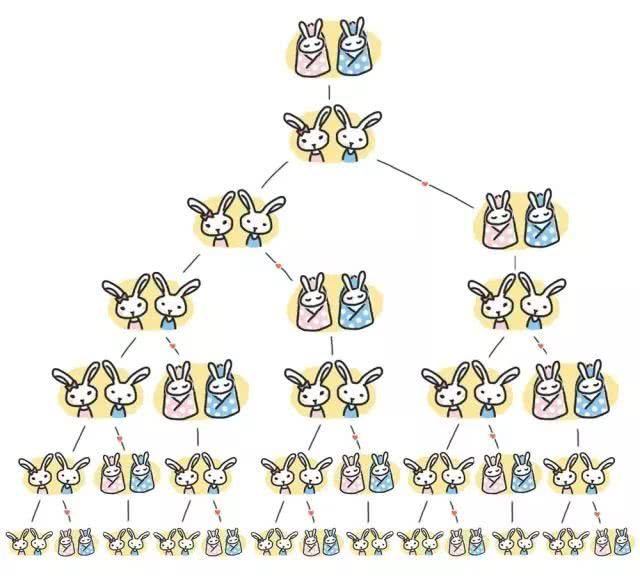
\includegraphics[scale=0.5]{img/C11/11-4/1.png}
\end{figure}

\begin{lstlisting}[style=htmlcssjs]
var n = 10;
var num1, num2, val;
var str = "";

if(n == 1) {
    console.log("1");
} else if(n == 2) {
    console.log("1, 1");
} else {
    num1 = 1;
    num2 = 1;
    str = "1, 1";
    for(var i = 3; i <= n; i++) {
        val = num1 + num2;
        str += ", " + val;
        num1 = num2;
        num2 = val;
    }
    console.log(str);
}
\end{lstlisting}

\begin{tcolorbox}
	\mybox{运行结果} \\
	1, 1, 2, 3, 5, 8, 13, 21, 34, 55
\end{tcolorbox}

\subsection{嵌套循环}

循环也可以进行嵌套使用。 \\

\mybox{九九乘法表} \\

\begin{table}[H]
	\centering
	\setlength{\tabcolsep}{1.5mm}{
		\begin{tabular}{|c|c|c|c|c|c|c|c|c|}
			\hline
			1*1=1 & 1*2=2  & 1*3=3  & 1*4=4  & 1*5=5  & 1*6=6  & 1*7=7  & 1*8=8  & 1*9=9  \\
			\hline
			2*1=2 & 2*2=4  & 2*3=6  & 2*4=8  & 2*5=10 & 2*6=12 & 2*7=14 & 2*8=16 & 2*9=18 \\
			\hline
			3*1=3 & 3*2=6  & 3*3=9  & 3*4=12 & 3*5=15 & 3*6=18 & 3*7=21 & 3*8=24 & 3*9=27 \\
			\hline
			4*1=4 & 4*2=8  & 4*3=12 & 4*4=16 & 4*5=20 & 4*6=24 & 4*7=28 & 4*8=32 & 4*9=36 \\
			\hline
			5*1=5 & 5*2=10 & 5*3=15 & 5*4=20 & 5*5=25 & 5*6=30 & 5*7=35 & 5*8=40 & 5*9=45 \\
			\hline
			6*1=6 & 6*2=12 & 6*3=18 & 6*4=24 & 6*5=30 & 6*6=36 & 6*7=42 & 6*8=48 & 6*9=54 \\
			\hline
			7*1=7 & 7*2=14 & 7*3=21 & 7*4=28 & 7*5=35 & 7*6=42 & 7*7=49 & 7*8=56 & 7*9=63 \\
			\hline
			8*1=8 & 8*2=16 & 8*3=24 & 8*4=32 & 8*5=40 & 8*6=48 & 8*7=56 & 8*8=64 & 8*9=72 \\
			\hline
			9*1=9 & 9*2=18 & 9*3=27 & 9*4=36 & 9*5=45 & 9*6=54 & 9*7=63 & 9*8=72 & 9*9=81 \\
			\hline
		\end{tabular}
	}
	\caption{九九乘法表}
\end{table}

\begin{lstlisting}[style=htmlcssjs]
var str = "";

for(var i = 1; i <= 9; i++) {
    for(var j = 1; j <= 9; j++) {
        str += i + "*" + j + "=" + i*j + "\t";
    }
    str += "\n";
}
console.log(str);
\end{lstlisting}

\mybox{输出图案}

\begin{lstlisting}
*
**
***
****
*****
\end{lstlisting}

\begin{lstlisting}[style=htmlcssjs]
var str = "";

for(var i = 1; i <= 5 i++) {
    for(var j = 1; j <= i; j++) {
        str += "*";
    }
    str += "\n";
}
console.log(str);
\end{lstlisting}

\newpage

\section{break or continue?}

\subsection{循环控制}

循环控制语句的作用是控制当前的循环结构是否继续向下执行,如果不进行控制,那么会根据既定的结构重复执行。如果有一些特殊的情况导致循环的执行中断,就称为循环的控制语句。循环控制语句的关键字有break和continue。 \\

break的作用是跳出当前循环,执行当前循环之后的语句。break只能跳出一层循环,如果是嵌套循环,那么需要按照嵌套的层次,逐步使用break来跳出。break语句只能在循环体内和switch语句内使用。 \\

continue的作用是跳过本轮循环,开始下一轮循环的条件判断。continue终止当前轮的循环过程,但它并不跳出循环。 \\

\mybox{break} \\

\begin{lstlisting}[style=htmlcssjs]
var str = "";

for(var i = 1; i <= 10; i++) {
    if(i == 5) {
        break;
    }
    str += i + " ";
}

console.log(str);
\end{lstlisting}

\begin{tcolorbox}
	\mybox{运行结果} \\
	1 2 3 4 
\end{tcolorbox}

\mybox{continue} \\

\begin{lstlisting}[style=htmlcssjs]
var str = "";

for(var i = 1; i <= 10; i++) {
    if(i == 5) {
        continue;
    }
    str += i + " ";
}

console.log(str);
\end{lstlisting}

\begin{tcolorbox}
	\mybox{运行结果} \\
	1 2 3 4 6 7 8 9 10
\end{tcolorbox}

\newpage